\section{Ground Truth}\label{sec:ground-truth}
In this section we introduce a ground truth to establish that both black-box analysis from \autoref{ch:Blackbox} and white-box analysis from 
\autoref{ch:Whitebox} conceptually work. 

To do so we design multiple configurable systems that test both analyses in different scenrios, afterwards we evaluate
them using \hyperref[researchQuestions]{research questions \ref*{researchQuestions}}. Since we design these systems ourselves we have 
a baseline that we use to manually build a \perfInfluenceModel for each system. All the different system will be designed with different focuses in mind
such as, a system that includes multicollinearity to see in what extent they influence the analyses.

As our first system we use the code from our previous example in \autoref{lst:performanceExample} and provide an additional feature model of the system in 
\autoref{fig:feature_abcd}. 

\begin{figure}[h]
    \centering
    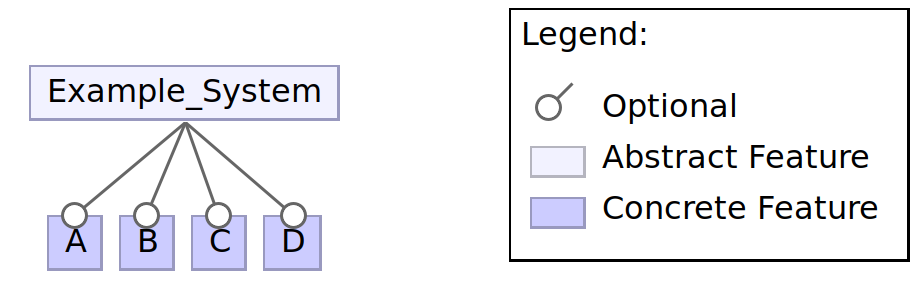
\includegraphics[scale=0.55]{gfx/Feature_ABCD.png}
    \caption{Feature model of \autoref{lst:performanceExample}.}
    \label{fig:feature_abcd}
\end{figure}

%Baseline and Blackbox
Out of \autoref{lst:performanceExample} and \autoref{fig:feature_abcd} we build \autoref{alg:xml-abcd} and declare all the feature variables. The baseline 
{\perfInfluenceModel} for this system is shown in \autoref{equ:performanceExamplePIMBaseline} and the {\perfInfluenceModel} build with the black-box
analysis data using multiple linear regression is shown in \autoref{equ:performanceExamplePIMBlackBox}. 

We analyse \autoref{lst:performanceExample} using our white-box analysis, this produces a TEF report file in \autoref{rep:tef-abcd},
afterwards we use this report to calculate the time spend in each feature region described as in \autoref{math:coefficients} and \autoref{math:time}.
This produces the following file in \autoref{alg:aggr-tef-abcd}, from which we build the following {\perfInfluenceModel}:

\begin{equation}
    \Pi = 2 + 1 \cdot A + 2 \cdot B + 1 \cdot C + 2 \cdot D + 2 \cdot A \cdot B + 0 \cdot C \cdot D
\end{equation}

We group our results in to compare them with each other.

\begin{table}[H]
    \centering
    \begin{tabular}{llllllll}
    \hline
    $\Pi$    & Base & A & B & C & D & A $\land$ B & C $\land$ D  \\ \hline
    Baseline & 2    & 1 & 2 & 1 & 2 & 2           & 0            \\
    Black-box & 2    & 1 & 2 & 1 & 2 & 2           & 0           \\
    White-box & 2    & 1 & 2 & 1 & 2 & 2           & 0           \\ \hline
    \end{tabular}  
    \caption{Direct comparison between the baseline, black-box and white-box {\perfInfluenceModel} for \autoref{lst:performanceExample}}
\end{table}